\documentclass[11pt]{article}
\usepackage[scaled=0.92]{helvet}
\usepackage{geometry}
\geometry{letterpaper,tmargin=1in,bmargin=1in,lmargin=1in,rmargin=1in}
\usepackage[parfill]{parskip} % Activate to begin paragraphs with an empty line rather than an indent %\usepackage{graphicx}
\usepackage{amsmath,amssymb, mathrsfs, dsfont}
\usepackage{tabularx}
\usepackage[font=footnotesize,labelfont=bf]{caption}
\usepackage{graphicx}
\usepackage{xcolor}
%\usepackage[linkbordercolor ={1 1 1} ]{hyperref}
%\usepackage[sf]{titlesec}
\usepackage{natbib}
\usepackage{../../Tianpei_Report}
%\usepackage{appendix}
%\usepackage{algorithm}
%\usepackage{algorithmic}

%\renewcommand{\algorithmicrequire}{\textbf{Input:}}
%\renewcommand{\algorithmicensure}{\textbf{Output:}}



\begin{document}
\title{Lecture 3: Inference in Tabular-based Graphical Models}
\author{ Tianpei Xie}
\date{ Aug. 25th., 2022 }
\maketitle
\tableofcontents
\newpage
\allowdisplaybreaks
\section{Background knowledge}
Recall the formulation of Bayesian network and Markov network
\begin{itemize}
\item Given directed graph $\cG=(\cV, \cE)$, where $(s,t) \neq (t,s)$, the \textbf{directed graphical model}  factorizes the joint distribution into a set of \emph{factors} $\{p_s(x_s | x_{\pi(s)}): s\in \cV\}$ according to the ancestor relations defined in $\cG$
\begin{align}
p(x_1, \ldots, x_{m}) &= \prod_{s \in \cV}p_s(x_s | x_{\pi(s)}). \label{eqn: dag_graph_factorization}
\end{align} This class of models are also referred as \emph{\textbf{Bayesian networks}} \citep{koller2009probabilistic}.


\item Given undirected graph $\cG=(\cV, \cE)$, where $(s,t) = (t,s)$, the joint distribution of \textbf{Markov random fields} (\textbf{Markov network}) \emph{factorize} as
\begin{align}
p(x_1, \ldots, x_{m}) &= \frac{1}{Z}\prod_{C \in \cC}\psi_{C}(x_{C}),\label{eqn: mrf_graph_factorization}
\end{align} where $Z$ is a constant chosen to ensure that the distribution is normalized. The set $\cC$ is often taken to be the \emph{set of all \textbf{maximal cliques} of the graph}, i.e., the set of cliques that are \emph{not} properly contained within any other clique. Note that any representation based on nonmaximal cliques can always be converted to one based on maximal cliques by redefining the compatibility function on a maximal clique to be the \emph{product} over the compatibility functions on the \emph{subsets} of that clique.

\item The canonical representation of \underline{\emph{\textbf{exponential famlity}}} of distribution has the following form
\begin{align}
p(x_1, \ldots, x_{m}) = p(\mb{x}; \mb{\eta}) &= \exp\paren{\inn{\mb{\eta}}{\mb{\phi}(\mb{x})} - A(\mb{\eta})}h(\mb{x})\nu(d\mb{x}) \nonumber \\
&= \exp\paren{\sum_{\alpha}\eta_{\alpha}\phi_{\alpha}(\mb{x}) -  A(\mb{\eta})} \label{eqn: exp_fam}
\end{align} where $\phi$ is a feature map  and $\mb{\phi}(\mb{x})$ defines a set of \emph{\textbf{sufficient statistics}} (or \emph{\textbf{potential functions}}). The normalization factor is defined as
\begin{align*}
 A(\mb{\eta}) &:= \log \int \exp\paren{ \inn{\mb{\eta}}{\mb{\phi}(\mb{x})} }h(\mb{x})\nu(d\mb{x}) = \log Z(\mb{\eta})
\end{align*} $A(\mb{\eta})$ is also referred as \textbf{\emph{log-partition function}} or \emph{cumulant function}. The parameters $\mb{\eta} = (\eta_{\alpha})$ are called \textbf{\emph{natural parameters}}  or \emph{canonical parameters}. The canonical parameter $\set{\eta_{\alpha}}$ forms a \textbf{natural (canonical) parameter space}
\begin{align}
\Omega = \set{\mb{\eta} \in \bR^{d}: A(\mb{\eta}) < \infty} \label{eqn: canonical_space}
\end{align}

\item The exponential family is the unique solution of \textbf{\emph{maximum entropy estimation}} problem:
\begin{align}
\min_{q \in \Delta}&\quad \kl{q}{p_{0}} \label{eqn: max_ent}\\
\text{s.t.}&\quad \E{q}{\phi_{\alpha}(X)} = \mu_{\alpha}\,\quad  \forall\, \alpha \in \cI   \label{eqn: max_ent_mean_constraint}
\end{align} where $\kl{q}{p_0} = \int \log(\frac{q}{p_0}) q dx = \E{q}{\log\frac{q}{p_0}}$ is the relative entropy or the Kullback-Leibler divergence of $q$ w.r.t. $p_0$.

Here $\mb{\mu} = (\mu_{\alpha})_{\alpha \in \cI}$ is a set of  \textbf{\emph{mean parameters}}. The space of mean parameters $\cM$ is a \emph{convex polytope} spanned by potential functions $\set{\phi_{\alpha}}$.
\begin{align}
\cM &:= \set{\mb{\mu} \in \bR^d: \exists q\,\; \text{s.t. } \E{q}{\phi_{\alpha}(X)} = \mu_{\alpha}\,\quad  \forall\, \alpha \in \cI} = \text{conv}\set{\phi_{\alpha}(x),\; x\in \cX, \;\alpha \in \cI}  \label{eqn: marginal_polytope}
\end{align}

\item Note that $A(\mb{\eta})$ is a convex function and its gradient $\grad{}{A}: \Omega \rightarrow \cM^{\circ}$ is a bijection between the natural parameter space $\Omega$ and the \underline{\textbf{interior}} of $\cM$,  $\cM^{\circ}$; $\grad{}{A}(\mb{\eta}) = \mb{\mu}$ based on the following equation 
\begin{align}
\partdiff{A}{\eta_{\alpha}} &= \E{\mb{\eta}}{\phi_{\alpha}(X)} := \int_{\cX^{m}}\phi_{\alpha}(\mb{x}) q(\mb{x}; \mb{\eta}) d\mb{x} = \mu_{\alpha} \label{eqn: partition_first_order}
\end{align}

\item Moreover $A(\mb{\eta})$ has a variational form 
\begin{align}
A(\mb{\eta}) &=  \sup_{\mb{\mu} \in \cM}\set{ \inn{\mb{\eta}}{\mb{\mu}} - A^{*}(\mb{\mu})} \label{eqn: log_partition_variational_form}
\end{align}
where $A^{*}(\mb{\mu})$ is the conjugate dual function of $A$ and it is defined as
\begin{align}
A^{*}(\mb{\mu}) &:= \sup_{\mb{\eta} \in \Omega} \set{\inn{\mb{\mu}}{\mb{\eta}} - A(\mb{\eta})} \label{eqn: conjugate_dual_partition}
\end{align}

It is shown that $A^{*}(\mb{\mu})  = -H(q_{\mb{\eta}(\mb{\mu})})$ for $\mb{\mu} \in  \cM^{\circ}$ which is the negative entropy. $A^{*}(\mb{\mu})$ is also the optimal value for the \textbf{maximum likelihood estimation} problem on $p$. The exponential family can be reparameterized according to its mean parameters $\mb{\mu}$ via backward mapping $(\grad{}{A})^{-1}: \cM^{\circ} \rightarrow  \Omega$, called \textbf{mean parameterization}.

\item We can formulate the \textbf{KL divergence} between two distributions in exponential family $\Omega$ using its primal and dual form
\begin{itemize}
\item \textbf{Primal-form}: given $\mb{\eta}_1, \mb{\eta}_2 \in \Omega$
\begin{align}
\kl{p_{\mb{\eta}_1}}{p_{\mb{\eta}_2}} \equiv  \kl{\mb{\eta}_1}{\mb{\eta}_2}
&=  A(\mb{\eta}_2) - A(\mb{\eta}_1) -  \inn{\mb{\mu}_{1}}{\mb{\eta}_2 - \mb{\eta}_1}  \label{eqn: kl_primal}\\
&\equiv  A(\mb{\eta}_2) - A(\mb{\eta}_1) -  \inn{\grad{}{A}(\mb{\eta}_1)}{\mb{\eta}_2 - \mb{\eta}_1}  \nonumber
\end{align}

\item \textbf{Primal-dual form}: given $\mb{\mu}_1 \in \cM, \mb{\eta}_2 \in \Omega$
\begin{align}
 \kl{\mb{\mu}_1}{\mb{\eta}_2} &= A(\mb{\eta}_2) + A^{*}(\mb{\mu}_1) - \inn{\mb{\mu}_{1}}{\mb{\eta}_2}  \label{eqn: kl_primal_dual}
\end{align}

\item \textbf{Dual-form}: given $\mb{\mu}_1, \mb{\mu}_2  \in \cM$
\begin{align}
 \kl{\mb{\mu}_1}{\mb{\mu}_2} &= A^{*}(\mb{\mu}_1) - A^{*}(\mb{\mu}_{2}) - \inn{\mb{\eta}_2}{\mb{\mu}_{1} - \mb{\mu}_{2}}  \label{eqn: kl_dual} \\
 &\equiv  A^{*}(\mb{\mu}_1) - A^{*}(\mb{\mu}_{2}) - \inn{\grad{}{A^{*}}(\mb{\mu}_{2})}{\mb{\mu}_{1} - \mb{\mu}_{2}} \nonumber
\end{align}
\end{itemize}
\end{itemize}


\section{Inference in graphical models}
Given a probability distribution $p$ defined by a graphical model, our focus will be solving one or more of the following computational inference problems:
\begin{enumerate}
\item \emph{Computing the likelihood of \textbf{observed data}}. $p(\mb{y}; \mb{\eta}) = \sum_{\mb{x}}p((\mb{y}; \mb{x}, \mb{\eta})$

\item \emph{Computing the \textbf{marginal distribution} $p(\mb{x}_{A})$ over a particular subset $A \subset \cV$ of nodes}.

\item \emph{Computing the \textbf{conditional distribution} $p(\mb{x}_{A} | \mb{x}_{B})$, for \textbf{disjoint} subsets $A$ and $B$, where $A \cup B$ is in general a proper
subset of $\cV$}. $p(\mb{x}_{A} | \mb{x}_{B}) = \frac{p(\mb{x}_{A} , \mb{x}_{B})}{p(\mb{x}_{B})}$

\item \emph{Computing a \textbf{mode} of the density (i.e., an element $\mb{x}$ in the set $\argmax_{\mb{x}\in \cX^m} p(\mb{x})$}.
\end{enumerate}

The problem $1-3$ are similar in that it all requires to compute the marginal distribution $p(\mb{x}_{A})$, which involves \textbf{summation} or \textbf{integration} depending on the factor form. In contrast, the problem of computing modes stated in $4$ is fundamentally different, since it entails \textbf{maximization} rather than integration. 

A \textbf{fundamental challenge} in graphical model is the \emph{high-dimensionality} of domain, which prohibits a simple integration and summation over the entile space. Therefore, inference on graphical model usually takes advantage of the \underline{\textbf{recursive structures}} within in the graph topology $\cG$. By utilizing recursive structure of graph, efficient algorithms such as \emph{\textbf{dynamic programming}} can be implemented.

\section{Inference for tabular-based graphical models}
The  tabular-based graphical models store information \emph{locally} via factors. In order to perform marginalization over the whole graph $\cG$,  adjacent factors need to \emph{\textbf{communicate}} with each other in order to make sure that they \textbf{agree on} the marginal distribution information on their \textbf{shared common variables}, i.e. \underline{\textbf{\emph{local consistency}}}. This communication is usually performed \textbf{in parallel}. Whether or not the \underline{\textbf{\emph{global consistency}}} can be reached via local consistency depends on the \textbf{\emph{graph topolgy}}. This affects the exactness of inference.  

For tree-based models, we can prove that the \textbf{\emph{local consistency}} \emph{is equal to} \textbf{\emph{global consistency}}.  This means that \textbf{exact inference} can be achieved via belief propagation at convergence. For general graphs, we transforms it into \emph{\textbf{junction trees}} and perform belief propagtion on junction trees.


%For tabular representation of factors, it is assumed that the graphical models are \textbf{discrete} and the \textbf{size} ($=$ dimensionality of domain $\times$ dimensionality of factor) of factors is  \textbf{small} so that summation or maximization \emph{\textbf{within each factor}} is a \emph{feasible} operation. The \textbf{key idea} for inference on tabular factors is to \textbf{propagate local information} gathered within each factor to the entire graph. 

%Here we consider two tasks:
%\begin{itemize}
%\item Computing the \emph{marginal distribution} $p(\mb{x}_{A})$ over a particular subset $A \subset \cV$ of nodes.
%
%\item Computing a \emph{mode} of the density (i.e., an element $\mb{x}$ in the set $\argmax_{\mb{x}\in \cX^m} p(\mb{x})$.
%\end{itemize}

\section{Exact marginal inference on tree-structure model}
\begin{figure}
\begin{minipage}[t]{1\linewidth}
  \centering
  \centerline{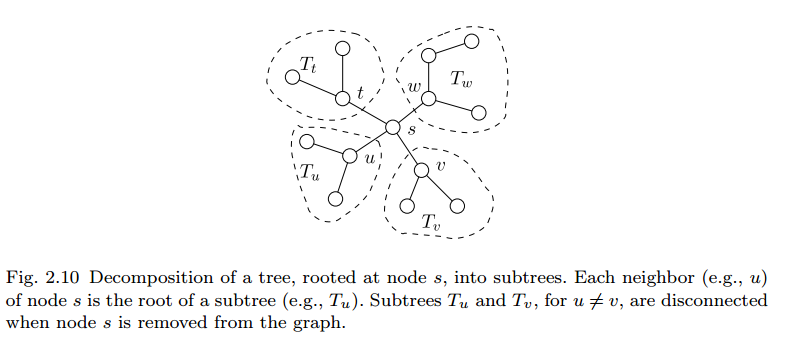
\includegraphics[scale = 0.5]{tree_decomp.png}}
\end{minipage}
\caption{\footnotesize{\textbf{The decomposition of trees by subtrees rooted at neighborhood.}}}
\label{fig: tree_decomp}
\end{figure}
\subsection{Sum-product belief propagation}
For tree-based graphical model, we can simplify the representation \eqref{eqn: mrf_graph_factorization} as
\begin{align}
p(x_1, \ldots, x_{m}; \cT) &= \frac{1}{Z}\prod_{s\in \cV}\psi_{s}(x_{s})\prod_{(s,t) \in \cE_{\cT}}\psi_{s,t}(x_{s}, x_{t}), \label{eqn: mrf_tree_factorization}
\end{align} In \textbf{marginalization} task, the target is to find marginal distribution
\begin{align}
\mu_{s}(x_{s}) &:= \sum_{\mb{x}_{-s}}p(x_s, \mb{x}_{-s}) \label{eqn: mrf_tree_marginal}
\end{align} where $\mb{x}_{-s} = [x_k]_{k\neq s}$. Since \eqref{eqn: mrf_tree_factorization} is a pruduct of all factors, the marginalization task is the \textbf{sum of products} among all factors over $\mb{x}_{-s}$.


As stated above, a tree $\cT = (\cV, \cE_{\cT})$ has clear a \textbf{recursive structure}. Specifically, define the neighborhood of node $s$ as
\begin{align*}
\cN(s) &= \set{t\in \cV: (s,t) \in \cE_{\cT} }
\end{align*} For each $u \in \cN(s)$, let $\cT_u = (\cV_u, \cE_u)$ be the subgraph formed by the set of nodes (and edges joining them) that \emph{can be reached from} $u$ by \textbf{paths} that \emph{\textbf{do not pass}} through node $s$. An \textbf{important property} for tree is that the subgraph $\cT$ is a tree and  for any $u\neq t,  \forall u,t \in \cN(s)$, $\cT_{u} \cap \cT_{t} = \emptyset$.  This means that we can \textbf{decompose} the tree $\cT_{s}$ rooted at $s$, by \textbf{removing} $s$ from the tree. It then form a collection or non-overlapping subtrees $\{\cT_t, t \in \cN(s)\}$. Figure \ref{fig: tree_decomp} shows the tree decomposition. 


%From this \textbf{tree decomposition property}, we can see that the same algorithm that runs in $\cT_{s}$ can also be applied to $\cT_{t}$ for all $t \in \cN(s)$. On the other hand, we can formulate the recursive algorithm that runs \textbf{locally} in each sub-trees $\cT_{t}$ and then in node $s$ to gather information to compute the global information on $\cT_{s}$. 

In particular, we introduce the \underline{\textbf{\emph{Sum-Product algorithm}}}, a form of \emph{\textbf{nonserial dynamic programming}} \citep{bertele1973non}, which generalizes the usual serial form of deterministic dynamic programming \citep{bertsekas2012dynamic} to arbitrary tree-structured graphs. The essential idea is divide and conque: dividing the problem of marginalization over \textbf{all variables} into the problem of marginalization over \textbf{local variables within each factor}; and 
"\textbf{passing}" this marginalized probability as "\textbf{\emph{message}}" to other nodes in the neigborhood.  See that
\begin{align}
\mu_{s}(x_{s}) &= p(x_s)\sum_{\mb{x}_{-s}}p(\mb{x}_{-s}|x_s)  \nonumber\\
&= p(x_s)\sum_{\mb{x}_{-s}}\prod_{t\in \cN(s)}p_{t}(\mb{x}_{\cV_{t}}|x_s; \cT_{t})\quad (\text{since }x_{\cV_{u}} \indep x_{\cV_{v}} | x_s\, \forall u,v \in \cN(s)) \nonumber\\
&= p(x_s)\prod_{t\in \cN(s)}\brac{\sum_{\mb{x}_{\cV_{t}}}p_{t}(\mb{x}_{\cV_{t}}|x_s; \cT_{t})}\quad (\text{ distribution law }) \nonumber
\end{align}

Define the \textbf{value function} that encodes the \emph{local information} to \textbf{be passed} from subtree $\cT_{t} \rightarrow s$ as a \underline{\textbf{\emph{message}}}
\begin{align}
M_{t \rightarrow s}^{*}(x_s) := M_{t,s}^{*}(x_s) &= \sum_{\mb{x}_{\cV_t}}\psi_{s,t}(x_s, x_t)\underline{p(\mb{x}_{\cV_t}; \cT_{t})} \label{eqn: mrf_tree_sum_product_message} 
\end{align} where $p(\mb{x}_{\cV_t}; \cT_{t})$ is the joint distribution of subtree $\cT_t$ following the same factorization as \eqref{eqn: mrf_tree_factorization}
\begin{align*}
p(\mb{x}_{\cV_t}; \cT_{t}) &=  \frac{1}{Z}\prod_{u\in \cV_t}\psi_{u}(x_{u})\prod_{(u,v) \in \cE_{\cT_t}}\psi_{u,v}(x_{u}, x_{v}).
\end{align*}  Given all messages $\{ M_{t,s}^{*}(x_s) \}_{t\in \cN(s)}$ from neighboring subtrees $\{\cT_t, t \in \cN(s)\}$, the \textbf{\emph{marginal distribution}} can be seen as a \underline{\textbf{value function} \textbf{at node}} $s$ as well: 
\begin{align}
\mu_{s}(x_{s}) &=\psi_{s}(x_s)\prod_{t \in \cN(s)}M_{t,s}^{*}(x_s). \label{eqn: mrf_tree_sum_product_marginal} 
\end{align} For subtree $\cT_t$, the computation of message $M_{t,s}^{*}(x_s)$ is again a sub-problem of marginalization. We can see that $(\mu_{s}(x_{s}),  (M_{t,s}^{*}(x_s))_{t \in \cN(s)})$ are all value functions which store local results for the problem.

Applying the decomposition twice and combing \eqref{eqn: mrf_tree_sum_product_message} and \eqref{eqn: mrf_tree_sum_product_marginal}, we can obtain the \underline{\textbf{\emph{Bellman equation}}} w.r.t. the \underline{\textbf{message function}} $M_{t,s}^{*}(x_s)$
\begin{align}
M_{t,s}^{*}(x_s) &= \sum_{\mb{x}_{\cV_t}}\psi_{s,t}(x_s, x_t)p(\mb{x}_{\cV_t}; \cT_{t}) \nonumber\\
&= \kappa \sum_{x_t \in \cX}\set{\psi_{s,t}(x_s, x_t)\psi_{t}(x_t)\prod_{u \in \cN(t) - \set{s}}M_{u,t}^{*}(x_t)}, \,  \forall t\in \cN(s),  s \in \cV \label{eqn: mrf_tree_sum_product_bellman_equation}
\end{align} where $\kappa > 0$ again denotes a \emph{normalization constant}. 


The \textbf{Sum-Product} algorithm is described as
\begin{enumerate}
\item At each iteration, each node $t$ \textbf{passes a message} $M_{t, u}^{*}(x_u)$ to \textbf{each of its neighbors} $u \in \cN(t)$. $M_{t,u}^{*}(x_u)$ is  a function of the possible states $x_u \in  \cX_u$ (i.e., a vector of length $|\cX_u|$ for discrete random variables).

This operation is done \textbf{in parallel} for all $t$. There are total of $2|\cE|$ messages in transmission.

\item Then the mssages from $t\rightarrow s$ are updated based on messages $u\rightarrow t$ from neighboring nodes $u \in \cN(t) - \set{s}$
\begin{align*}
M_{t,s}^{*}(x_s) &\leftarrow \kappa \sum_{x_t \in \cX}\set{\psi_{s,t}(x_s, x_t)\psi_{t}(x_t)\prod_{u \in \cN(t) - \set{s}}M_{u,t}^{*}(x_t)},
\end{align*} 

\item Repeat the above steps until converge
\end{enumerate}
The algorithm will \textbf{converge to fixed-point solution} $M^{*} := \set{M_{t,s}^{*}, M_{s, t}^{*}, (s,t)\in \cE_{\cT}}$ for tree-structured graphs after a finite number of iterations. This solution is the solution of Bellman equation \eqref{eqn: mrf_tree_sum_product_bellman_equation}. Since the fixed point $M_{t,s}^{*}$ specifies the solution to all of the subproblems, the marginal $\mu_s$ at every node $s \in  \cV$ can be computed easily via equation \eqref{eqn: mrf_tree_sum_product_marginal}.

Specifically, for tree-based graphical model, the sum-product iteration is done via \textbf{forward-backward procedue}, i.e. starting \textbf{from root} passing messages down to \textbf{leaves} \textbf{requesting} marginal probability information; and then  \textbf{from leaf} passing message up to \textbf{root} \textbf{filling} in marginal probability information. The sum-product algorithm is also known as \underline{\textbf{\emph{belief propagation algorithm}}} \citep{wainwright2008graphical}.

\subsection{Factor graph message passing}
\begin{figure}
\begin{minipage}[t]{1\linewidth}
  \centering
  \centerline{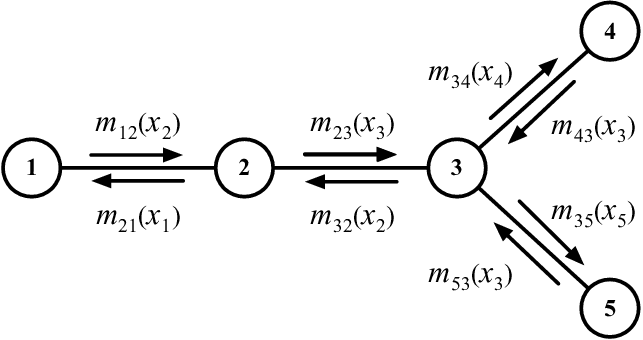
\includegraphics[scale = 0.3]{belief_prop.png}}
\end{minipage}
\caption{\footnotesize{\textbf{The sum-product message passing, i.e. belief propagation.}}}
\label{fig: tree_decomp}
\end{figure}

In \textbf{\emph{factor-graph}} formulation, the definitions of \textbf{variable node} and \textbf{factor node} are introduced. The joint probability is factorized into product of factors.
\begin{align}
p(x_1, \ldots, x_{m}) &= \frac{1}{Z}\prod_{a \in \cC}\psi_{a}(\mb{x}_{a}),\label{eqn: mrf_graph_factor}
\end{align}

The message in \eqref{eqn: mrf_tree_sum_product_message} is split into \textbf{two messages}.
\begin{enumerate}
\item \textbf{Messages from a variable node $t$ to a factor node $a$}: 
\begin{align}
M_{t\rightarrow a}(x_t) &= \prod_{a' \in \cN(t) - \set{s}}M_{a' \rightarrow t}(x_t) \label{eqn: message_var_to_factor}
\end{align} Note that in factor graph, the neighborhood of a variable node $\cN(t)$ only contains factor nodes, thus $a'$ is a factor node and $M_{a' \rightarrow t}$ is a message from factor to variable.

\item \textbf{Messages from a factor node $a$ to a variable node $t$}: It is defined to be the product of the factor with messages from all other nodes, marginalized over all variables except the one associated with $t$
\begin{align}
M_{a \rightarrow t}(x_t) &= \sum_{\mb{x}_{a. -t}}\set{\psi_{a}(\mb{x}_{a,-t}, x_t)\prod_{w \in \cN(a) - \set{t}}M_{w \rightarrow s}(x_w)}  \label{eqn: message_factor_to_product}
\end{align} Here $\cN(a)$ only contains variable node so $M_{w \rightarrow s}$ is the message from variable node $w$ to factor $s$. Also $\mb{x}_{a, -t} = (x_{w}, w \in \cN(a) - \set{t})$ denote all input of factor $a$ except for variable $x_t$.
\end{enumerate} Note that for tree, each (edge) factor only contains two nodes, and each node only connects to two (edge) factors. So these two messages are combined. 

The marginal distribution of node $s$, $\mu_s(x_s)$
\begin{align*}
\mu_s(x_s) &\propto \prod_{a \in \cN(s)}M_{a \rightarrow s}(x_s)
\end{align*} and the marginal distribution of $\mb{x}_a$ belongs to factor $a$
\begin{align*}
\mu_a(\mb{x}_a) &\propto \psi_{a}(\mb{x}_{a})\prod_{t \in \cN(a)}M_{t \rightarrow a}(x_t)
\end{align*}

\subsection{Bellman equation in log-space}
The Bellman equation in  \eqref{eqn: mrf_tree_sum_product_bellman_equation} with tabular factor $\psi$ is for all $x_s \in \cX, t\in \cN(s), s\in \cV$. It is a system of $2|\cE| \times |\cX|$ linear equations. For tree structure, $|\cV| = |\cE| + 1$. Let $|\cV| =d$, $|\cX| = r$, then $\mb{m}= [M_{t,s}^{*}(x_s)]_{\forall (s,t)\in \cE, x_s\in \cX} \in \bR^{2(d-1)r}$. We can replace the Bellman equation with two steps
\begin{align*}
H_{s,t}(x_s, x_t) &= \psi_{s,t}(x_s, x_t)\psi_{t}(x_t)\prod_{u \in \cN(t) - \set{s}}M_{u,t}^{*}(x_t) \\
M_{t,s}^{*}(x_s) &= \sum_{x_t}H_{s,t}(x_s, x_t) 
\end{align*} and then introduce the logarithm $h_{s,t}(x_s, x_t) = \log H_{s,t}(x_s, x_t) $ and $m_{s,t}(x_s) = \log M_{t,s}^{*}(x_s) $. We have Bellman equation in log-space
\begin{align}
h_{s,t}(x_s, x_t) &= \log  \psi_{s,t}(x_s, x_t) + \log \psi_{t}(x_t) + \sum_{u \in \cN(t) - \set{s}}  m_{u,t}(x_t) \label{eqn: mrf_tree_sum_product_bellman_equation_log_factor}\\
m_{t,s}^{*}(x_s) &= \log\paren{\sum_{x_t \in \cX}\exp(h_{s,t}(x_s, x_t))} := \text{soft-max}_{x_t}\paren{h_{s,t}(x_s, x_t)}  \label{eqn: mrf_tree_sum_product_bellman_equation_log_message}\\
\Rightarrow m_{t,s}^{*}(x_s) &= \text{soft-max}_{x_t \in \cX}\brac{\log  \psi_{s,t}(x_s, x_t) + \log \psi_{t}(x_t) + \sum_{u \in \cN(t) - \set{s}}  m_{u,t}(x_t)}  \label{eqn: mrf_tree_sum_product_bellman_equation_log}
\end{align} Here the log-sum-exp function is a \textbf{smooth version of maximum} $\log(\sum_t e^{h_t}) = \text{soft-max}_{t}(h)$.



\section{Exact mode inference on tree-structure model}
The problem of finding a \textbf{mode} of a tree-structured distribution is formulated as
\begin{align}
\max_{\mb{x}\in \cX^m} & \frac{1}{Z}\prod_{s\in \cV}\psi_{s}(x_{s})\prod_{(s,t) \in \cE_{\cT}}\psi_{s,t}(x_{s}, x_{t})  \label{eqn: mode_finding} 
\end{align}

Similar to Sum-Product algorithm, we have \underline{\textbf{Max-Product algorithm}} where maximization replaces the summation. Max-Product algorithm is essentially a \emph{\textbf{generalized Viterbi algorithm}}. We consider the problem  to compute the \underline{\textbf{\emph{max-marginal}}}
\begin{align}
\nu_{s}(x_{s}) &:= \max_{\mb{x}_{-s}}p(x_s, \mb{x}_{-s}) \label{eqn: mrf_tree_mode}\\
&= p(x_s)\max_{\mb{x}_{-s}}p(\mb{x}_{-s}|x_s) \nonumber \\
&= p(x_s)\max_{\mb{x}_{-s}}\prod_{t\in \cN(s)}p_{t}(\mb{x}_{\cV_{t}}|x_s; \cT_{t})\quad (\text{by tree decomposition}) \nonumber\\
&= p(x_s)\prod_{t\in \cN(s)}\brac{\max_{\mb{x}_{\cV_{t}}}p_{t}(\mb{x}_{\cV_{t}}|x_s; \cT_{t})}\quad (\text{monotonicity of maximum}) \nonumber
\end{align} 
So from \eqref{eqn: mrf_tree_sum_product_message}, we see that the \textbf{value functions} are defined as 
\begin{align}
M_{t \rightarrow s}^{*}(x_s) := M_{t,s}^{*}(x_s) &= \max_{\mb{x}_{\cV_t}}\;\psi_{s,t}(x_s, x_t)\;\underline{p(\mb{x}_{\cV_t}; \cT_{t})} \label{eqn: mrf_tree_max_product_message} \\
\nu_{s}(x_{s}) &= \psi_{s}(x_s)\prod_{t \in \cN(s)}M_{t,s}^{*}(x_s). \label{eqn: mrf_tree_max_product_marginal} 
\end{align}

Following similar derivation as \eqref{eqn: mrf_tree_sum_product_bellman_equation},  we have the \textbf{Bellman equation} for \textbf{max-product} algorithm:
\begin{align}
M_{t,s}^{*}(x_s) &= \max_{x_t}\set{\psi_{s,t}(x_s, x_t)\psi_{t}(x_t)\prod_{u \in \cN(t) - \set{s}}M_{u,t}^{*}(x_t)}\quad \forall t\in \cN(s),\; s \in \cV \label{eqn: mrf_tree_max_product_bellman_equation}
\end{align} For HMM, since there are only one input $u=t-1$ besides $t+1$ in the neighborhood of $t$,  $M_{t,t+1}^{*}(x_{t+1}) = \max_{x_t}M_{(t-1),t}^{*}(x_t)\; \psi_{t, t+1}(x_t, x_{t+1})\psi_{t}(x_t)$. This is the objective of Viterbi decoding.

\section{Junction tree representation}
\begin{figure}
\begin{minipage}[t]{1\linewidth}
  \centering
  \centerline{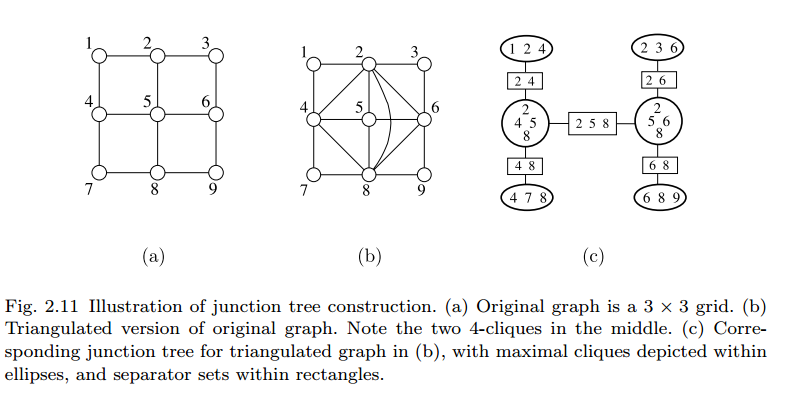
\includegraphics[scale = 0.5]{triangulation_junction_tree.png}}
\end{minipage}
\caption{\footnotesize{\textbf{Triangulation and junction tree. \citep{wainwright2008graphical}}}}
\label{fig: triangulation_junction_tree}
\end{figure}
Given a graph with cycles, a natural idea is to cluster its nodes so as to form a \emph{\textbf{clique tree}} -- that is, an \emph{acyclic} graph whose \emph{nodes} are formed by the \emph{maximal cliques} of $\cG$. In order to apply the message passing algorithm to clique trees, a clique tree satisfy an additional restriction so as to ensure \textbf{correctness} of these computations.  In particular, since a given vertex $s \in \cV$ may appear in multiple cliques (say $C_1$ and $C_2$), what is required is a mechanism for enforcing \underline{\textbf{\emph{consistency}}} among the different appearances of the variable $x_s$. It turns out that the following property is \emph{\textbf{necessary} and \textbf{sufficient}} to enforce such consistency:
\begin{definition}
A clique tree has the \underline{\textbf{\emph{running intersection property}}} if for any two clique nodes $C_1$ and $C_2$, all nodes on the unique path joining them \emph{contain the intersection} $C_1 \cap C_2$. A clique tree with this property is known as a \emph{\textbf{junction tree}}.
\end{definition}

Junction tree can be constructed using \emph{\textbf{triangulation}}. We say that a graph is \underline{\emph{\textbf{triangulated}}} if every cycle of length \emph{four} or longer has a \emph{chord}, meaning an edge joining a pair of nodes that are not adjacent on the cycle.  

The following is the \textbf{key theorem} behind the junction tree algorithm.
\begin{theorem}\citep{jordan2003introduction, wainwright2008graphical}\\
For an undirected graph, $\cG$, the following properties are \emph{equivalent}:
\begin{itemize}
\item Graph $\cG$ is \underline{\textbf{triangulated}}.
\item The clique graph of $\cG$ has a \underline{\textbf{junction tree}}.
\item There is an \underline{elimination ordering} for $\cG$ that does not lead to any added edges.
\end{itemize}
\end{theorem} See Figure \ref{fig: triangulation_junction_tree} for construction of junction tree via triangulation.


This result underlies the  \underline{\textbf{\emph{junction tree algorithm}}}  \citep{jordan2003introduction} for exact inference on \emph{arbitrary graphs}:
\begin{enumerate}
\item Given a graph with cycles $\cG$, \emph{\textbf{triangulate}} it by adding edges as necessary.

\item Form a \emph{\textbf{junction tree}} associated with the triangulated graph $\tilde{\cG}$.

\item Run a \emph{\textbf{tree inference}} algorithm on the junction tree.
\end{enumerate}

To describe the inference on junction tree, we need to introduce potential functions not only on the cliques in the junction tree, but also on the \emph{\textbf{separators}} in the junction tree. A \emph{separator} $S= C_1 \cap C_2$ is the intersections of cliques that are \emph{adjacent} in the junction tree. Let $\phi_{C}(\cdot)$ denote a potential function defined over the subvector $\mb{x}_C = (x_t, t \in C)$ on clique $C$, and let $\phi_{S}(\cdot)$ denote a potential on a separator $S$. 

\begin{figure}
\begin{minipage}[t]{1\linewidth}
  \centering
  \centerline{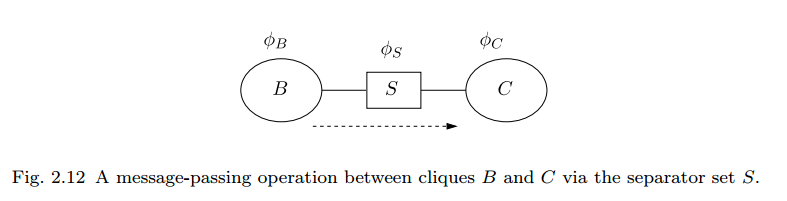
\includegraphics[scale = 0.5]{message_passing_separator.png}}
\end{minipage}
\caption{\footnotesize{\textbf{Message passing through seperator clique.}}}
\label{fig: message_passing_separator}
\end{figure}

We \textbf{initialize} the clique potentials by assigning each \emph{compatibility function} in the original graph to (exactly) one \emph{clique potential} and taking the \textbf{product} over these compatibility functions. The separator potentials are initialized to \textbf{unity}.
\begin{align*}
\phi_{C}(\mb{x}_{C}) &\leftarrow \prod_{c \subset C}\psi_{c}(\mb{x}_c) \\
\phi_{S}(\mb{x}_{S}) &\leftarrow 1  
\end{align*}


Given this set-up, the basic \textbf{message-passing} step of the junction tree algorithm are given by
\begin{align}
\widetilde{\phi}_{S}(\mb{x}_{S}) &\leftarrow \sum_{\mb{x}_{B - S}}\phi_{B}(\mb{x}_{B}) \label{eqn: junction_tree_message_passing_separator}\\
\phi_{C}(\mb{x}_{C}) & \leftarrow \frac{\widetilde{\phi}_{S}(\mb{x}_{S}) }{\phi_{S}(\mb{x}_{S})}\phi_{C}(\mb{x}_{C}) \label{eqn: junction_tree_message_passing_clique}
\end{align} The above describe the message passing from clique $B$ to clique $C$, as illustrated in Figure \ref{fig: message_passing_separator}. 

It can be verified that if a message is passed from $B$ to $C$, and subsequently from $C$ to $B$, then the resulting clique potentials are consistent with each other, meaning
that \textbf{they agree} with respect to the vertices $S$.

\newpage
\bibliographystyle{plainnat}
\bibliography{book_reference.bib}
\end{document}